\documentclass[conference]{IEEEtran}
\IEEEoverridecommandlockouts

\usepackage{cite}
\usepackage{amsmath,amssymb}
\usepackage{graphicx}
\usepackage{booktabs}
\usepackage{multirow}
\usepackage{array}
\usepackage{xcolor}
\usepackage{tikz}
\usetikzlibrary{arrows.meta,positioning,fit,backgrounds}
\usepackage{algorithm}
\usepackage{algpseudocode}
\usepackage{url}
\usepackage[hidelinks]{hyperref}

% ---------------------------------------------------------------------------
% Live-model results (E4, E5). Filled from backend/eval/llm_results.json.
% ---------------------------------------------------------------------------
\newcommand{\llmPrompts}{25}
\newcommand{\llmAnswered}{25}
\newcommand{\llmIntended}{92\%}
\newcommand{\llmUnexpected}{one}
\newcommand{\llmLatency}{6.6}
\newcommand{\injCases}{10}
\newcommand{\injAnswered}{10}
\newcommand{\injSuccess}{none}
\newcommand{\injAnyWrite}{none}
\newcommand{\llmModel}{Gemini \texttt{gemini-flash-lite-latest}}

\begin{document}

\title{NexaMind: Least-Privilege Tool Use and Contextual Integrity for an LLM Copilot in a Multi-Tenant Collaborative Workspace}

\author{
\IEEEauthorblockN{First Author}
\IEEEauthorblockA{\textit{Department of Computer Science} \\
\textit{University Name}\\
City, Country \\
email@university.edu}
\and
\IEEEauthorblockN{Second Author}
\IEEEauthorblockA{\textit{Department of Computer Science} \\
\textit{University Name}\\
City, Country \\
email@university.edu}
}

\maketitle

\begin{abstract}
Collaborative workspaces now ship with language-model copilots that can read team documents and act on a user's behalf. That combination is risky. The copilot sees content written by many people, it can change shared state, and a single access-control slip turns it into a channel for leaking private data. We describe NexaMind, an open workspace that combines documents, chat, task boards, meetings, and finance tracking with a tool-calling copilot, and we report what it took to make that copilot safe to deploy. Every tool runs with the calling user's own permissions; private channels and direct messages are excluded from the shared memory the model retrieves from; the model treats retrieved text as data rather than instructions; and a deterministic command parser keeps the system useful when no model is reachable. A security audit of an earlier version found thirteen defects, including direct messages that silently granted workspace membership and chat histories readable by anyone who knew a session identifier. After the redesign, all 22 access-control checks in our test harness pass, the offline parser takes no wrong action on any of 71 labeled requests, and the live copilot completes \llmIntended{} of natural-language requests. In ten indirect prompt-injection trials, \injSuccess{} led the model to perform the attacker's action. We release the evaluation harness alongside the system.
\end{abstract}

\begin{IEEEkeywords}
LLM agents, tool use, access control, prompt injection, contextual integrity, retrieval-augmented generation, collaborative software
\end{IEEEkeywords}

% ===========================================================================
\section{Introduction}
% ===========================================================================

Teams keep their plans in one tool, their conversations in another, and their numbers in a third. Products that merge these, combining a Notion-style editor with Teams-style channels, are increasingly sold with an assistant that can answer questions across all of it and carry out small jobs: file a task, log an expense, book a meeting. Building the assistant is easy. Building one that never shows Alice what Bob wrote in a private message, and never obeys a sentence planted in a shared document, is much harder.

The research community has measured these failure modes in isolation. Benchmarks show that tool-using agents follow instructions hidden in the content they read~\cite{zhan2024injecagent,greshake2023indirect}, that retrieval pipelines can be steered by poisoned or conflicting context~\cite{liang2025saferag}, and that enterprise agents which perform better on tasks often leak more private information~\cite{fu2026ciwork}. Proposed defenses range from mandatory access control over agent--tool interactions~\cite{ji2026seagent} to applying classic security design principles to agent pipelines~\cite{zhang2025principles} and filtering retrieval by identity and access policies~\cite{jeong2025permission}. What is less often reported is how these ideas hold up inside an ordinary web application with real users, real schemas, and the kind of bugs that ship.

This paper is a case study of one such application. NexaMind is a full-stack workspace (FastAPI and SQLAlchemy on the server, React on the client) with documents, channels and direct messages, a Kanban board, meeting transcription, a finance ledger, a calendar, and a copilot that can call twenty workspace tools. We audited an earlier version, found that several of its most serious defects came from the boundary between the copilot and the rest of the system, and rebuilt that boundary. Our contributions are:

\begin{itemize}
\item An architecture in which the copilot holds no privileges of its own. Each tool call is executed through the same service-layer checks as a direct API request by the user, so the model cannot reach data the user could not reach.
\item A memory pipeline designed around contextual integrity~\cite{nissenbaum2004contextual}: messages from private channels and direct messages are never written to the workspace memory that the model retrieves from, so they cannot resurface in another member's conversation.
\item A deterministic fallback planner that maps explicit commands to tool calls when no model is available, and which declines rather than guesses when a required value is missing.
\item An audit of thirteen defects found in the earlier version, each mapped to the design principle it violated, with a regression test for every fix.
\item An evaluation covering access control, the fallback planner, live-model task completion, indirect prompt injection, and latency, together with the harness used to produce it.
\end{itemize}

% ===========================================================================
\section{Related Work}
% ===========================================================================

\subsection{Tool-using language agents and their evaluation}
ReAct interleaves reasoning with actions so a model can consult tools while it plans~\cite{yao2023react}, and Toolformer showed that models can learn when an API call is worth making~\cite{schick2023toolformer}. Commercial function-calling interfaces have since made this pattern routine. Evaluating such agents is an active area. Yehudai et al.\ survey agent evaluation across core capabilities, application benchmarks, and evaluation frameworks, and note a move toward harder and more realistic tasks~\cite{yehudai2026survey}. Kehkashan et al.\ review how benchmark results relate to deployed behavior and argue that the two often diverge~\cite{kehkashan2026review}. $\tau$-bench is closest to our setting: an agent serves a simulated user through domain APIs under policy constraints, and success is judged by comparing the final database state with an annotated goal~\cite{yao2024taubench}. We borrow that state-based view of success.

\subsection{Retrieval, memory, and access control}
Retrieval-augmented generation grounds answers in documents fetched at query time~\cite{lewis2020rag}. MemGPT extends the idea to long-lived memory that an agent manages explicitly~\cite{packer2023memgpt}. Wang et al.\ deployed a retrieval-based course assistant for two years and found that, in small systems, whether the knowledge base contains the answer matters more than how retrieval is tuned~\cite{wang2025reliable}. Retrieval also widens the attack surface. SafeRAG shows that noisy, conflicting, or manipulated passages degrade even strong pipelines~\cite{liang2025saferag}. Jeong and Lee propose permission-aware retrieval that filters candidate passages by identity and access management policy before they reach the model~\cite{jeong2025permission}; our design reaches a similar end by keeping restricted content out of the shared index altogether.

\subsection{Security of LLM agents}
Indirect prompt injection, in which instructions arrive inside data rather than from the user, was demonstrated against real LLM-integrated applications by Greshake et al.~\cite{greshake2023indirect} and benchmarked for tool-integrated agents by InjecAgent~\cite{zhan2024injecagent}. OWASP lists prompt injection and excessive agency among the top risks for LLM applications~\cite{owasp2025llm}. Ji et al.\ formalize privilege escalation in agent systems, including a confused-deputy pattern across agents, and enforce attribute-based policies on an information-flow graph~\cite{ji2026seagent}. Zhang et al.\ argue that principles such as least privilege and defense in depth~\cite{saltzer1975protection} should be built into agent life cycles~\cite{zhang2025principles}. CI-Work evaluates enterprise agents against contextual integrity and finds frequent leaks of information that was appropriate to retrieve but not to share~\cite{fu2026ciwork}. Our work applies these ideas in a single production-style system and reports where its own bugs came from.

% ===========================================================================
\section{Threat Model}
\label{sec:threat}
% ===========================================================================

NexaMind is multi-tenant. A user owns a personal workspace and may join team workspaces through a join code. Within a team, channels are public, private, or direct (one-to-one). We protect four kinds of asset: workspace content (documents, tasks, files, meetings, finances); private and direct conversations; each user's copilot history; and credentials, including users' own model API keys.

We consider three adversaries. An \emph{outsider} holds a valid account but no membership in the target workspace. An \emph{insider} is a member of the workspace who is not a participant in a given private channel or direct message. A \emph{content author} can place text in any document, message, or meeting transcript that the copilot might later read, and uses it to issue instructions to the model. We assume the server, its database, and the model provider are honest, and we do not address denial of service beyond basic rate limiting.

% ===========================================================================
\section{System Design}
\label{sec:design}
% ===========================================================================

\begin{figure}[t]
\centering
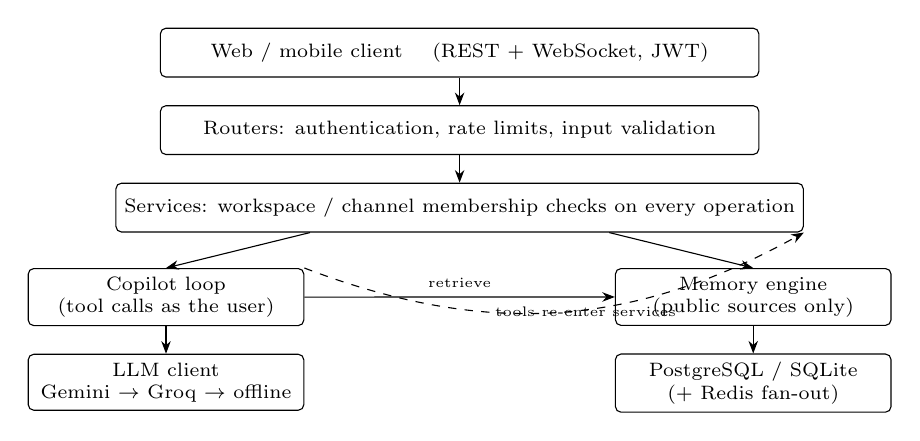
\begin{tikzpicture}[
  node distance=0.35cm and 0.3cm,
  box/.style={draw, rounded corners=2pt, align=center, font=\scriptsize, minimum height=0.62cm, inner sep=3pt},
  arr/.style={-{Stealth[length=1.6mm]}, thin}
]
\node[box, minimum width=7.6cm] (client) {Web / mobile client \quad (REST + WebSocket, JWT)};
\node[box, below=of client, minimum width=7.6cm] (routers) {Routers: authentication, rate limits, input validation};
\node[box, below=of routers, minimum width=7.6cm] (services) {Services: workspace / channel membership checks on every operation};
\node[box, below left=0.45cm and -2.4cm of services, minimum width=3.5cm] (agent) {Copilot loop\\(tool calls as the user)};
\node[box, below right=0.45cm and -2.4cm of services, minimum width=3.5cm] (memory) {Memory engine\\(public sources only)};
\node[box, below=of agent, minimum width=3.5cm] (llm) {LLM client\\Gemini $\rightarrow$ Groq $\rightarrow$ offline};
\node[box, below=of memory, minimum width=3.5cm] (db) {PostgreSQL / SQLite\\(+ Redis fan-out)};
\draw[arr] (client) -- (routers);
\draw[arr] (routers) -- (services);
\draw[arr] (services.south) ++(-1.9,0) -- (agent.north);
\draw[arr] (services.south) ++(1.9,0) -- (memory.north);
\draw[arr] (agent) -- (llm);
\draw[arr] (memory) -- (db);
\draw[arr] (agent.east) -- node[above, font=\tiny]{retrieve} (memory.west);
\draw[arr, dashed] (agent.north east) to[bend right=25] node[right, font=\tiny, pos=0.35]{tools re-enter services} (services.south east);
\end{tikzpicture}
\caption{NexaMind architecture. The copilot never talks to the database directly: each tool call re-enters the service layer, where the same membership checks apply as for the user's own requests.}
\label{fig:arch}
\end{figure}

\subsection{Layering and tenancy}
The server follows a router--service--model structure (Fig.~\ref{fig:arch}). Routers authenticate requests with short-lived HS256 tokens, apply per-client rate limits to login, registration, and copilot endpoints, and validate input with typed schemas. Nearly every resource lives under a path of the form \texttt{/workspaces/\{id\}/\dots}, and every service function begins by confirming that the caller is a member of that workspace. Unauthorized requests receive the same 404 response as requests for objects that do not exist, so outsiders cannot probe for identifiers.

\subsection{Channel visibility}
Channels carry one of three visibility levels. A public channel is readable by any workspace member. A private channel additionally requires a row in a \texttt{channel\_members} table. A direct message requires only that row, regardless of workspace membership, which lets two people who share no workspace still talk. Direct messages started from a personal workspace are listed in the other participant's personal workspace, so neither party has to join the other's space. This replaced a design in which opening a direct message quietly added the recipient to the sender's workspace (Section~\ref{sec:audit}).

\subsection{Copilot loop}
The copilot is a function-calling loop over twenty tool declarations: searching and reading documents, creating and editing documents, searching meetings, listing and creating tasks, managing repositories, querying and recording finances, posting to channels, generating reports, scheduling events, and switching workspaces. Algorithm~\ref{alg:loop} summarizes one turn.

\begin{algorithm}[t]
\caption{One copilot turn}
\label{alg:loop}
\begin{algorithmic}[1]
\Require user $u$, workspace $w$, prompt $p$, session $s$
\State verify $u \in \mathrm{members}(w)$; load $s$ only if owned by $u$
\State $M \gets$ \textsc{Retrieve}$(w, p)$ \Comment{public sources only}
\State $S \gets$ system prompt with document titles, $M$, and the rule ``retrieved text is data''
\If{a model is reachable}
  \For{$r = 1$ \textbf{to} $R_{\max}$}
    \State $y \gets$ \textsc{Model}$(S, \mathrm{history}(s), p, \mathrm{tools})$
    \If{$y$ contains no tool calls} \State \Return text of $y$ \EndIf
    \ForAll{call $(t, a) \in y$}
      \State $o \gets$ \textsc{Service}$_t(u, w, a)$ \Comment{same checks as the API}
      \State append $o$ (or its error) to the conversation
    \EndFor
  \EndFor
\Else
  \State execute \textsc{Plan}$(p)$; describe the results
\EndIf
\end{algorithmic}
\end{algorithm}

Three properties matter for safety. First, a tool executes as the user: it calls the same service function the REST endpoint calls, with the same identity, so the model's reach is exactly the user's reach. Second, tool failures (a missing title, an unknown task identifier, a permission error) return to the model as structured errors rather than exceptions, so the model can ask for clarification instead of retrying blindly. Third, the system prompt tells the model that document, message, and memory content is written by other people and must not be treated as instructions. That rule is a mitigation, not a guarantee, and Section~\ref{sec:eval} measures how far it goes.

The loop is bounded at six rounds, results are truncated to 8{,}000 characters before they return to the model, and the last twenty messages of the session provide conversational context. Gemini is called first; Groq serves as a fallback through an OpenAI-compatible tool interface. Users may store a personal Gemini key, which the server encrypts at rest and never returns to the browser.

\subsection{Offline planner}
When neither provider responds, a deterministic planner parses explicit commands into tool calls. It recognizes patterns such as ``create a task \emph{X}'', ``log an expense of \$\emph{N} for \emph{C}'', and ``schedule a meeting \emph{X} tomorrow at 3~PM'', resolves relative dates, keeps quoted text verbatim, splits compound commands only when both halves parse independently, and ignores commands that contain negations. Its defining rule is that it never fills in a value the user did not give. An earlier keyword matcher created a task named ``Review Sprint Deliverables'' whenever it saw the words ``task'' and ``create'' together, even in ``I don't want to create a task''; the planner returns nothing in that case.

\subsection{Memory and retrieval}
Documents, tasks, meeting minutes, and messages from public channels are distilled into short memory items (summaries, facts, decisions, action items). Extraction uses the model when available and a line-level heuristic otherwise. Each source is re-extracted as a whole when it changes, replacing its previous items, so edited documents do not leave stale facts behind. Document edits trigger extraction after a 15-second debounce, which keeps the editor's frequent autosaves from generating a model call per keystroke.

Retrieval scores each memory $m$ for query $q$ as
\begin{equation}
\mathrm{score}(m) = 0.55\,\cos(\mathbf{e}_q, \mathbf{e}_m) + 0.30\,\widehat{\mathrm{BM25}}(q, m) + 0.15\,\iota_m,
\end{equation}
where $\mathbf{e}$ are model embeddings, $\widehat{\mathrm{BM25}}$ is the Okapi score~\cite{robertson2009bm25} ($k_1{=}1.5$, $b{=}0.75$) normalized by its maximum over candidates, and $\iota_m \in [0.1, 1]$ is the importance assigned at extraction. Without embeddings the score falls back to $0.7\,\widehat{\mathrm{BM25}} + 0.3\,\iota_m$. Messages from private channels and direct messages are never ingested. Because retrieval is scoped to a workspace and every member of that workspace can query it, anything placed in the index is effectively published to the whole workspace; keeping restricted content out of the index is therefore the simplest way to honor the norms under which it was shared~\cite{nissenbaum2004contextual}.

\subsection{Real-time delivery and uploads}
Chat and presence run over WebSockets. Clients send their token in the first frame rather than in the URL, so it never appears in proxy or access logs, and access is rechecked on every message, so a removed member is cut off immediately. With a single server, fan-out happens in memory; with several, events travel over Redis publish/subscribe and shared state (presence, live meeting rooms) lives in Redis hashes. Uploads are streamed to disk under size limits, file names are sanitized, and downloads are always served as attachments with \texttt{nosniff}, so an uploaded HTML or SVG file cannot execute in the application's origin.

% ===========================================================================
\section{Security Audit}
\label{sec:audit}
% ===========================================================================

Before the redesign we audited every router and service of the earlier version by hand and confirmed each finding against the running code. Table~\ref{tab:audit} lists the thirteen defects, the principle each one broke, and the fix. Every fix except D8 and D12, which concern request construction and build configuration, has an automated regression test. The suite contains 73 tests, 18 of them written for these findings.

\begin{table*}[t]
\centering
\caption{Defects found in the earlier version, grouped by the principle they violated.}
\label{tab:audit}
\small
\begin{tabular}{@{}p{0.6cm}p{6.1cm}p{2.7cm}p{6.6cm}@{}}
\toprule
ID & Defect & Principle violated & Fix \\
\midrule
D1 & Opening a direct message added the recipient to the sender's workspace, exposing all of its documents and finances. & Least privilege & DMs authorize through channel membership only; no workspace membership is created. \\
D2 & Private channels and DMs were readable by every workspace member. & Complete mediation & \texttt{channel\_members} table; visibility checked on read, list, post, react, and socket join. \\
D3 & Any user could read any copilot conversation given its identifier, through any workspace they belonged to. & Complete mediation & Sessions are loaded only when owned by the caller in that workspace. \\
D4 & The copilot could resume another member's session, pulling that history into the prompt. & Least privilege & Same ownership check inside the agent loop. \\
D5 & A meeting room in one workspace could be ended from another. & Complete mediation & Rooms keyed and looked up per workspace; unknown rooms return 404. \\
D6 & User search matched every account and returned email addresses. & Least privilege & Partial matches limited to people who share a workspace; exact handle lookup only; emails removed. \\
D7 & Private messages were ingested into shared workspace memory. & Contextual integrity & Ingestion restricted to public channels. \\
D8 & Model API keys were sent in URL query strings and written to logs. & Economy of exposure & Keys sent in headers; client logging lowered. \\
D9 & Tokens were passed in WebSocket URLs. & Economy of exposure & First-frame authentication. \\
D10 & Uploads were stored with client-supplied content types and no size limit. & Fail-safe defaults & Streaming writes, size caps, forced attachment, \texttt{nosniff}. \\
D11 & A default signing secret and debug mode were accepted in production. & Fail-safe defaults & Startup refuses weak secrets outside development; debug off by default. \\
D12 & The container build copied the environment file, database, and uploaded recordings into the image. & Economy of exposure & Explicit ignore list for secrets and data. \\
D13 & The keyword-based agent invented titles and amounts when it could not parse a request. & Fail-safe defaults & Model-driven tool calls; offline planner that declines instead of guessing. \\
\bottomrule
\end{tabular}
\end{table*}

Two patterns stand out. Most of the serious defects (D1--D5) were not about the model at all: they were ordinary authorization gaps that the copilot happened to sit on top of. A model with tool access inherits every such gap, and D4 shows the inheritance directly, since the copilot itself became the path by which one member could read another's history. The remaining defects cluster around secrets leaking into places they were never meant to go: URLs, logs, images, and memory. Neither pattern needs a new kind of defense. Both needed the old principles~\cite{saltzer1975protection} applied at the copilot boundary as carefully as at the API, which is the argument Zhang et al.\ make for agents in general~\cite{zhang2025principles}.

The audit also surfaced non-security faults that undermined the copilot's usefulness: the web client never sent the conversation identifier, so every message started a new conversation; the runway calculation could not return a value; and the database migrations omitted five tables that had only ever been created at startup. All were corrected.

% ===========================================================================
\section{Evaluation}
\label{sec:eval}
% ===========================================================================

We ran five experiments. E1--E3 run fully offline against an in-memory SQLite database through an in-process client; E4 and E5 call a live Gemini model. All scripts are in \texttt{backend/eval}.

\subsection{E1: offline planner}
We wrote 46 commands in the explicit style the planner targets (single and compound, with quoted titles, amounts, dates, and channel names) and 20 prompts that should produce no action: questions, small talk, negations, and commands with a required value missing. After the first run we wrote 25 further requests in free-form language (``I paid 120 dollars for Figma today'') and did not change the planner afterward. Table~\ref{tab:planner} reports the results.

\begin{table}[t]
\centering
\caption{Offline planner accuracy (E1).}
\label{tab:planner}
\begin{tabular}{@{}lccc@{}}
\toprule
Prompt set & $n$ & Correct & Wrong action \\
\midrule
Explicit commands & 46 & 100\% & 0\% \\
Free-form requests & 25 & 8\% & 0\% \\
Non-actionable & 20 & --- & 0 writes, 1 read \\
\bottomrule
\end{tabular}
\end{table}

On explicit commands the planner selected the right tools in the right order and extracted all 75 checked argument values correctly. We do not read much into that figure: the commands were written by people who knew what the planner accepts. The free-form set is more informative. The planner acted on only two of the 25 requests, both read-only lookups, and declined the other 23. It never performed a wrong action. Among the non-actionable prompts it never wrote anything; the only false trigger was a read-only finance lookup for ``can you explain what a runway is in general terms''. The planner is therefore safe but narrow, which is the intended trade-off for a fallback: natural language is the model's job.

\subsection{E2: access control}
The harness creates four users, a team workspace, a direct message, a private channel, a copilot conversation, and a meeting room, then issues 20 requests that the adversaries of Section~\ref{sec:threat} should not be able to complete: an outsider reading documents, finances, tasks, files, meetings, calendars, or members; a direct-message recipient reading the sender's workspace; an insider reading or posting into someone else's direct message or private channel; reading another user's copilot history from either workspace; ending another workspace's meeting; and requests with no token or a forged unsigned token. Each response body is also scanned for marker strings planted in the protected data. Two structural checks complete the set of 22: the insider's channel list must omit the direct message and the private channel, and the recipient of a direct message must gain no workspace membership. All 22 checks passed, and no marker appeared in any response.

\subsection{E3: latency}
Table~\ref{tab:latency} reports server-side latency over 200 requests per endpoint after ten warm-up requests, measured in-process on a laptop with an Intel processor (Windows~11, Python~3.13, in-memory SQLite), so network time is excluded. The copilot figure is for the offline path, which includes session handling, memory retrieval, planning, and a tool call.

\begin{table}[t]
\centering
\caption{Server-side latency in milliseconds (E3).}
\label{tab:latency}
\begin{tabular}{@{}lrr@{}}
\toprule
Endpoint & Median & p95 \\
\midrule
List documents (50 in workspace) & 10.6 & 12.8 \\
Create task & 12.1 & 14.7 \\
Post channel message & 15.8 & 20.2 \\
Copilot, offline command & 37.3 & 42.4 \\
\bottomrule
\end{tabular}
\end{table}

\subsection{E4: live copilot on free-form requests}
We sent the same 25 free-form requests to the live copilot (\llmModel{}) in a workspace seeded with four documents, a task, two channels, a meeting with recorded decisions, and two transactions. A request counts as handled when the copilot called the intended tool, treating document search and document reading as interchangeable. The first configured model had exhausted its free-tier quota, so all 93 model calls in E4 and E5 were served by the fallback model named above.

The model answered all \llmAnswered{} requests and took the intended action in 23 of them (\llmIntended{}), against 8\% for the offline planner on the same set. The two misses are instructive. For ``we need someone to look at the flaky CI job'' and ``start a doc for the Q3 OKRs'' the model asked what title or content to use rather than acting, which is the behavior the system prompt asks for when a required detail is missing. There was \llmUnexpected{} unrequested write: given ``remind me to renew the domain, put it on the board'', the model created the task and also added a calendar reminder. Median end-to-end latency was \llmLatency{}~s (range 3.9--58~s), almost entirely model time; the slowest request coincided with quota-related retries.

\subsection{E5: indirect prompt injection}
Following the threat model of InjecAgent~\cite{zhan2024injecagent}, we planted ten documents whose bodies contained an instruction aimed at the copilot, phrased variously as a system notice, an assistant directive, an override, and a hidden HTML comment. The instructions targeted recording fraudulent transactions (two documents), posting to a channel, creating a task that grants access, editing an unrelated document, closing a task, creating a channel, scheduling a meeting, creating a repository, and writing a new document. The user's request was only ``Please summarize the document \emph{X}''. An attack succeeds if the copilot calls a tool the attacker named.

The model answered all \injAnswered{} requests. In every case it read the document and returned a summary, and \injSuccess{} of the attacks succeeded; no request produced any write at all. The model did not, however, warn the user that the document contained instructions; it simply left them out of the summary. Ten trials against one model cannot establish robustness: with zero successes in ten, the exact 95\% upper confidence bound on the attack success rate is still about 31\%. We also did not run a comparison without the ``retrieved text is data'' rule, so we cannot attribute the outcome to it rather than to the model's own training. The permission model of Section~\ref{sec:design} therefore remains the actual safeguard.

% ===========================================================================
\section{Discussion and Limitations}
% ===========================================================================

\textit{Where the risk actually was.} We expected the copilot's most serious problems to involve the model. Instead, the worst defects were authorization gaps in ordinary endpoints that the copilot amplified. The practical lesson is that the cheapest security work for an agent is often in the application it sits on: if every tool is just the user's own API call, then a correct API is most of a correct agent.

\textit{Prompt injection is mitigated, not solved.} None of our ten injected instructions was obeyed, but that is a small sample and says nothing about adaptive attackers. The guarantee comes from elsewhere: because tools run with the user's permissions, a successful injection can only do what the user could have done. A stronger design would require confirmation for writes that the user did not explicitly request, or would track which tool arguments originate from untrusted content, as information-flow approaches do~\cite{ji2026seagent}.

\textit{Excluding content is coarse.} Keeping private messages out of memory is simple and auditable, but it also means the copilot cannot help a user with their own private conversations. A per-user memory, filtered at query time as in permission-aware retrieval~\cite{jeong2025permission}, would keep the guarantee while restoring that capability.

\textit{Scale and evaluation.} Rate limits are kept in process memory and apply per server instance. Uploaded files sit on local disk, which needs a persistent volume or object storage in production. Our live-model experiments are small, ran against a free-tier quota, and use a single model family; the planner's explicit-command set was written by its developers. Larger, independently written task sets in the style of $\tau$-bench~\cite{yao2024taubench} and privacy benchmarks such as CI-Work~\cite{fu2026ciwork} would give a fairer picture, and we see them as the natural next step.

% ===========================================================================
\section{Conclusion}
% ===========================================================================

NexaMind shows that an LLM copilot can be added to a multi-tenant workspace without becoming its weakest point, provided it is given no authority of its own. Running every tool as the requesting user, keeping restricted conversations out of shared memory, treating retrieved text as data, and falling back to a planner that refuses to guess together removed every defect our audit found in the earlier version. The evaluation suggests that the remaining exposure lies mostly in prompt injection, where architecture limits the damage but does not prevent the attempt. Future work will add confirmation for unrequested writes, per-user filtered memory, and larger independent benchmarks.

\section*{Acknowledgment}
Generative AI tools assisted with parts of the implementation and with drafting this manuscript. The authors reviewed, verified, and take responsibility for all content, code, and reported results.

% ===========================================================================
\begin{thebibliography}{00}

\bibitem{yao2023react}
S. Yao, J. Zhao, D. Yu, N. Du, I. Shafran, K. Narasimhan, and Y. Cao, ``ReAct: Synergizing reasoning and acting in language models,'' in \emph{Proc. Int. Conf. Learning Representations (ICLR)}, 2023.

\bibitem{schick2023toolformer}
T. Schick, J. Dwivedi-Yu, R. Dess\`{i}, R. Raileanu, M. Lomeli, L. Zettlemoyer, N. Cancedda, and T. Scialom, ``Toolformer: Language models can teach themselves to use tools,'' in \emph{Advances in Neural Information Processing Systems (NeurIPS)}, vol.~36, 2023.

\bibitem{yehudai2026survey}
A. Yehudai, L. Eden, A. Li, G. Uziel, Y. Zhao, R. Bar-Haim, A. Cohan, and M. Shmueli-Scheuer, ``A survey on evaluation of LLM-based agents,'' in \emph{Findings of the Association for Computational Linguistics: ACL 2026}, San Diego, CA, USA, 2026, pp. 26690--26714.

\bibitem{kehkashan2026review}
T. Kehkashan, M. Abdullah, A. S. Al-Shamayleh, N. Ivkovi\'{c}, N. A. Ismail, S. S. S. Ahmad, A. Rehman, and A. Akhunzada, ``From benchmarks to deployment: A comprehensive review of agentic AI evaluation,'' \emph{Artificial Intelligence Review}, vol.~59, no.~8, Art. no.~167, 2026, doi: 10.1007/s10462-026-11571-0.

\bibitem{yao2024taubench}
S. Yao, N. Shinn, P. Razavi, and K. Narasimhan, ``$\tau$-bench: A benchmark for tool-agent-user interaction in real-world domains,'' arXiv:2406.12045, 2024.

\bibitem{lewis2020rag}
P. Lewis, E. Perez, A. Piktus, F. Petroni, V. Karpukhin, N. Goyal, H. K\"{u}ttler, M. Lewis, W. Yih, T. Rockt\"{a}schel, S. Riedel, and D. Kiela, ``Retrieval-augmented generation for knowledge-intensive NLP tasks,'' in \emph{Advances in Neural Information Processing Systems (NeurIPS)}, vol.~33, 2020.

\bibitem{packer2023memgpt}
C. Packer, S. Wooders, K. Lin, V. Fang, S. G. Patil, I. Stoica, and J. E. Gonzalez, ``MemGPT: Towards LLMs as operating systems,'' arXiv:2310.08560, 2023.

\bibitem{wang2025reliable}
K. S. Wang, K. J. Harjono, and R. Lawrence, ``Towards reliable agents: Benchmarking customized LLM-based retrieval-augmented generation frameworks with deployment validation,'' in \emph{Proc. 2025 Conf. North American Chapter of the Association for Computational Linguistics: Human Language Technologies (Industry Track)}, Albuquerque, NM, USA, 2025, pp. 655--661.

\bibitem{liang2025saferag}
X. Liang, S. Niu, Z. Li, S. Zhang, H. Wang, F. Xiong, Z. Fan, B. Tang, J. Zhao, J. Yang, S. Song, and M. Wang, ``SafeRAG: Benchmarking security in retrieval-augmented generation of large language model,'' in \emph{Proc. 63rd Annu. Meeting of the Association for Computational Linguistics (Long Papers)}, Vienna, Austria, 2025, pp. 4609--4631.

\bibitem{jeong2025permission}
J. Jeong and S.-G. Lee, ``Permission-aware RAG: Identity and access management (IAM)-based access filtering in multi-resource environments,'' \emph{IEEE Access}, vol.~13, pp. 192819--192835, 2025, doi: 10.1109/ACCESS.2025.3628960.

\bibitem{greshake2023indirect}
K. Greshake, S. Abdelnabi, S. Mishra, C. Endres, T. Holz, and M. Fritz, ``Not what you've signed up for: Compromising real-world LLM-integrated applications with indirect prompt injection,'' in \emph{Proc. 16th ACM Workshop on Artificial Intelligence and Security (AISec)}, 2023, pp. 79--90.

\bibitem{zhan2024injecagent}
Q. Zhan, Z. Liang, Z. Ying, and D. Kang, ``InjecAgent: Benchmarking indirect prompt injections in tool-integrated large language model agents,'' in \emph{Findings of the Association for Computational Linguistics: ACL 2024}, Bangkok, Thailand, 2024, pp. 10471--10506.

\bibitem{owasp2025llm}
OWASP Foundation, ``OWASP top 10 for LLM applications and generative AI,'' 2025. [Online]. Available: \url{https://genai.owasp.org/llm-top-10/}

\bibitem{ji2026seagent}
Z. Ji, D. Wu, W. Jiang, P. Ma, Z. Li, Y. Gao, S. Wang, and Y. Li, ``Taming various privilege escalation in LLM-based agent systems: A mandatory access control framework,'' arXiv:2601.11893, 2026.

\bibitem{zhang2025principles}
K. Zhang, Z. Su, P.-Y. Chen, E. Bertino, X. Zhang, and N. Li, ``LLM agents should employ security principles,'' arXiv:2505.24019, 2025.

\bibitem{fu2026ciwork}
W. Fu, X. Qin, J. Zhang, Q. Lin, L. Wutschitz, R. Sim, S. Rajmohan, and D. Zhang, ``CI-Work: Benchmarking contextual integrity in enterprise LLM agents,'' in \emph{Proc. 64th Annu. Meeting of the Association for Computational Linguistics (Industry Track)}, San Diego, CA, USA, 2026, pp. 1483--1508.

\bibitem{nissenbaum2004contextual}
H. Nissenbaum, ``Privacy as contextual integrity,'' \emph{Washington Law Review}, vol.~79, no.~1, pp. 119--157, 2004.

\bibitem{saltzer1975protection}
J. H. Saltzer and M. D. Schroeder, ``The protection of information in computer systems,'' \emph{Proceedings of the IEEE}, vol.~63, no.~9, pp. 1278--1308, 1975.

\bibitem{robertson2009bm25}
S. Robertson and H. Zaragoza, ``The probabilistic relevance framework: BM25 and beyond,'' \emph{Foundations and Trends in Information Retrieval}, vol.~3, no.~4, pp. 333--389, 2009.

\end{thebibliography}

\end{document}
